\documentclass{bioinfo}
\copyrightyear{2012}
\pubyear{2012}
\raggedend
\setcounter{MaxMatrixCols}{24}

\begin{document}
\firstpage{1}

\title[Repressilator]{Repressilator: simulation and analysis of a synthetic oscillatory network in \textit{E. coli}}
\author[Standage]{Daniel S. Standage}
\address{Department of Genetics, Development, and Cell Biology, Iowa State University, Ames, IA 50011}

\history{March 26, 2012}

\maketitle

%\begin{abstract}
%Phasellus porta, diam eu egestas hendrerit, erat augue cursus quam, in sagittis massa dolor sed lacus. Praesent dictum sapien pellentesque nibh suscipit id dictum enim ornare. Aliquam enim magna, aliquet at ornare vitae, tempus non sapien. Aliquam erat volutpat. Praesent turpis nunc, rutrum sed hendrerit quis, accumsan quis turpis. Mauris elementum, sem eget posuere blandit, tellus metus dapibus dolor, vel accumsan sapien quam at mauris. In vel ornare massa. Donec sed erat nisi. Sed et mi nec lorem aliquet rutrum. Donec accumsan elementum ligula, in lobortis dolor consectetur sed. Integer suscipit dictum congue. Morbi ac risus nunc. Donec eu erat ut ligula accumsan sollicitudin. Nam gravida eros id risus placerat posuere.
%\end{abstract}

\section*{Background}

In a foundational paper in synthetic biology, \cite{Elowitz} describe the design and construction of the \textit{repressilator}, an artificial gene regulatory network. The authors designed a plasmid consisting of three transcription regulators each designed to repress the expression of another factor in a cyclic manner, forming a negative feedback loop. In computer simulations, the biochemical species of the network exhibit regular oscillatory behavior, and this behavior was confirmed by transforming the plasmid into \textit{Escherichia coli} cells along with another plasmid containing a reporter gene sensitive to one of the repressilator's species.  The fluorescence oscillations observed in \textit{E. coli} were independent of any naturally occurring biological clock.

This landmark study demonstrated that there is value not only in analyzing and inferring naturally existing networks, but also in designing and engineering synthetic networks to induce certain desired behaviors. The repressilator serves as a model for investigating naturally occurring biological oscillations (such as circadian rhythms). Furthermore, improved understanding of this network's properties can be beneficial for the design and engineering of larger, more complex biological systems with oscillatory components.

For this project, I performed a stochastic simulation of the repressilator network and was able to produce results very similar to those described by the original authors. I also performed some basic network analyses on the repressilator to compute elementary flux modes, extreme pathways, and minimal cut sets. A brief discussion of these analyses is given below.

\begin{figure}
  \begin{center}
    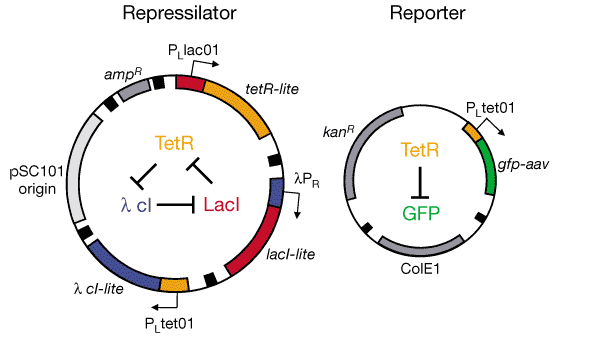
\includegraphics[width=240px]{../repressilator.png}
  \end{center}
  \caption{\cite{Elowitz} designed and constructed a synthetic network, termed the \textit{repressilator}, consisting of two plasmids. The first plasmid contains three genes (\textit{TetR}, $\lambda$ \textit{cI}, and \textit{LacI}), each encoding an transcription inhibitor. Each of the three inhibitors are designed to repress the expression of another, forming a cycle of negative repression. The second plasmid contains a reporter gene sensitive to \textit{TetR} concentration. After transforming \textit{Escherichia coli} with the repressilator, the authors reported periodic oscillations in \textit{TetR} concentrations independent of any natural biological clock found in \textit{E. coli}. This confirmed corresponding numerical simulations demonstrating the network's oscillatory behavior.}
\end{figure}

\section*{Simulation}

\cite{Elowitz} reported results for both a deterministic continuous simulation and a stochastic discrete simulation of the repressilator. Both simulations demonstrate regular oscillations in the concentration of the three proteins in the network, although the stochastic simulation (unsurprisingly) is a little less regular. For this project, I decided to reproduce the stochastic simulation. The simulation was implemented in Matlab using Gillespie's algorithm \citep{Gillespie}: source code is included in the appendix.

The stoichiometric matrix for the repressilator network, as shown below, is very simple.
\[
V_b = 
\begin{bmatrix}
1 & 0 & -1 & 0 & 0 & 0 & 0 & 0 & 0 & 0 & 0 & 0 \\
0 & 1 & 0 & -1 & 0 & 0 & 0 & 0 & 0 & 0 & 0 & 0 \\
0 & 0 & 0 & 0 & 1 & 0 & -1 & 0 & 0 & 0 & 0 & 0 \\
0 & 0 & 0 & 0 & 0 & 1 & 0 & -1 & 0 & 0 & 0 & 0 \\
0 & 0 & 0 & 0 & 0 & 0 & 0 & 0 & 1 & 0 & -1 & 0 \\
0 & 0 & 0 & 0 & 0 & 0 & 0 & 0 & 0 & 1 & 0 & -1 
\end{bmatrix}
\]
Each pair of rows corresponds to the mRNA and protein products of one of the 3 genes (6 total biomolecular species). Each set of 4 columns corresponds to the transcription and translation of the gene, as well as the degredation of the transcript and protein products (12 total reactions).

Evaluation of propensities relies on a variety of network parameters. Parameters for the simulation were selected from the repressilator network model contained in the BioModels network database \citep{Li}.

Gillespie's algorithm was run for 1000 iterations, and the simulated concentrations of the proteins were graphed (as shown in \textbf{Figure 2}).

\begin{figure}
  \begin{center}
    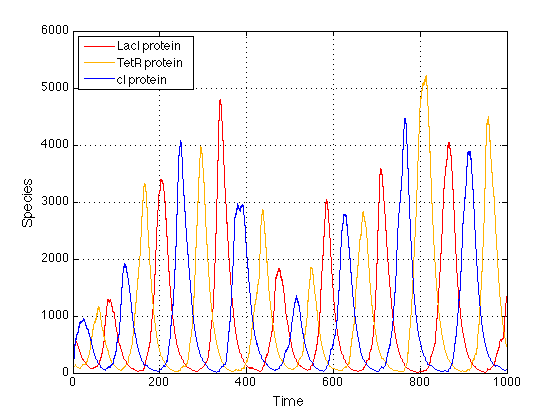
\includegraphics[width=240px]{../results.png}
  \end{center}
  \caption{Concentrations of the three primary network components (\textit{tetR}, $\lambda$ \textit{cI}, and \textit{lacI}) in a stochastic, discrete simulation of the \textit{repressilator} network. These inhibitors exhibit oscillatory behavior very similar to that shown in the original publication by \cite{Elowitz}.}
\end{figure}

\section*{Network analysis}
Two models of the repressilator were constructed \textit{in silico} for network analysis using CellNetAnalyzer \citep{Klampt}.

\subsection*{Basic model}
The basic model, taken directly from the Elowitz paper and the BioModels database, includes 6 biomolecular species and 12 reactions (as represented by the stoichiometric matrix $V_b$ above). The repressilator includes 3 inhibitors (\textit{tetR}, $\lambda$ \textit{cI}, and \textit{lacI}), and the 6 species of this model correspond to the mRNAs and proteins associated with each inhibitor. The 12 reactions correspond to the transcription, transcript degredation, translation, and protein degredation corresponding to each inhibitor.

\subsection*{Detailed model}
A second more detailed model was formulated in an attempt to 1) more realistically capture the biological complexity of the network, and 2) provide more interesting and substantial results than those given by analysis of the first (basic) network.

The detailed model incorporates additional characteristics of the inhibition mechanisms of the repressilator, increasing the number of biomolecular species from 6 to 15 and the number of reactions from 12 to 24. The 15 species of the model correspond to the following elements related to each of the 3 inhibitors: a gene with an unbound operator, a gene with a partially bound operator, a gene with a fully bound operator, an mRNA, and a protein. The 24 reactions of the of this model correspond to the following reactions related to each inhibitor: transcription from genes with unbound operators, transcription from genes with fully bound operators, binding of inhibitors to gene operators, decoupling of first inhibitor from gene operator, decoupling of second inhibitor from gene operator, translation, mRNA degredation, and protein degredation (see Figure 3). A stoichiometric matrix corresponding to this more detailed model is shown in the appendix.

\begin{figure}
  \begin{eqnarray*}
    D_{i} + 2 P_{j} &\rightarrow& F_{i} \\
              F_{i} &\rightarrow& H_{i} + P_{j} \\
              H_{i} &\rightarrow& D_{i} + P_{j} \\
                    &\rightarrow& R_{i} \\
                    &\rightarrow& R_{i} \\
                    &\rightarrow& P_{i} \\
              R_{i} &\rightarrow& \\
              P_{i} &\rightarrow& \\
  \end{eqnarray*}
  \caption{Chemical equations describing a more detailed model of the \textit{repressilator} network. Symbols in the equations have the following meaning: $D$ refers to DNA (gene with unbound operator), $H$ refers to ``half-bound" DNA (gene with partially bound operator), $F$ refers to ``fully-bound" DNA (gene with fully-bound operator), $R$ refers to mRNA (transcription product), $P$ refers to protein (translated and active inhibitor), $i$ is an element of the sequence $(tetR, cI, lacI)$, and $j$ is an element of the sequence $(lacI, tetR, cI)$. Overall, there are 15 biochemical species and 24 reactions in this more detailed model.}
\end{figure}

CellNetAnalyzer's network analysis features were used to mathematically characterize the network based on these two models.

\subsection*{Elementary modes and extreme pathways}
CellNetAnalyzer (CNA) identified 6 elementary flux modes in the basic model of the repressilator network. Each of these modes corresponds to the production and degredation of one of the 6 biomolecular species in the network, and simply has edge weights of $1.0$ on the edges corresponding to those reactions. CNA identified 6 extreme pathways as well: due to the network's simplicity and symmetry, each elementary mode is also an extreme pathway.

In the detailed repressilator model, CNA identified 12 elementary flux modes. There appeared to be some symmetry in these modes as well. For each of the 3 inhibitor pathways, there are 4 corresponding elementary flux modes: one related to binding and unbinding of inhibitors to gene operators, one related to transcription and degredation of mRNAs from genes with unbound (active) operators, one related to transcription and degredation of mRNAs from genes with bound (repressed) operators, and one related to translation and degredation of the inhibitor protein. Again, the edge weights of related reactions are $1.0$ and again, each elementary mode corresponds to a distinct extreme pathway.

Because this network is designed to be oscillatory, it did not make sense to optimize equilibrium flux for any particular network component.

\subsection*{Minimal cut sets}
For each elementary mode in the basic model, CNA identified 64 minimal cut sets, each involving 6 of the 12 reactions in the model. Again, due to the symmetry in the model, the 64 cut sets for each of the 6 modes were identical. For each elementary mode in the detailed model, CNA identified 1728 minimal cut sets, each involving 9 of the 24 reactions in the model. These 1724 cut sets were also identical for each of the 12 elementary flux modes.

\section*{Discussion}
Simulating the repressilator's kinetics and deriving results very similar to those published in the original paper was immensely satisfying. Because of the simplicity and symmetry of the network I chose for this assignment, however, the network analysis wasn't quite as exciting. Although my attempt to provide a more detailed model of the repressilator did not add much meaning to my network analyses, it \textit{was} a fruitful exercise. And repeating the network analysis steps multiple times gave me sufficient experience so that I will have no problems in the future using CNA to analyze more substantial networks.

Overall, I find the field of synthetic biology fascinating. If I were an engineer, this would definitely be my area of research interest!

\section*{Acknowledgement}
I'd like to thank Will Pett for his help with evaluating propensities, and to Tasos for his help and patience with CellNetAnalyzer.



%\bibliographystyle{natbib}
%\bibliographystyle{achemnat}
%\bibliographystyle{plainnat}
%\bibliographystyle{abbrv}
%\bibliographystyle{bioinformatics}
%
%\bibliographystyle{plain}
%
%\bibliography{Document}


\begin{thebibliography}{}
\bibitem[Elowitz and Leibler, 2000]{Elowitz} Elowitz, Michael B., and Stanislas Leibler (2000) A synthetic oscillatory network of transcriptional regulators. \textit{Nature}, \textbf{403}, 335-338.

\bibitem[Gillespie, 1976]{Gillespie} Gillespie, Daniel T. (1976). A General Method for Numerically Simulating the Stochastic Time Evolution of Coupled Chemical Reactions. \textit{Journal of Computational Physics}, \textbf{22}(4): 403�434.

\bibitem[Klampt \textit{et~al}, 2007]{Klampt} Klamt S, Saez-Rodriguez J and Gilles ED (2007) Structural and functional analysis of cellular networks with CellNetAnalyzer. \textit{BMC Systems Biology}, \textbf{1}:2.

\bibitem[Li \textit{et~al}, 2010]{Li} Li C, Donizelli M, Rodriguez N, Dharuri H, Endler L, Chelliah V, Li L, He E, Henry A, Stefan MI, Snoep JL, Hucka M, Le Nov�re N, Laibe C (2010) BioModels Database: An enhanced, curated and annotated resource for published quantitative kinetic models. \textit{BMC Systems Biology}, \textbf{4}:92.


\end{thebibliography}

%\newpage
\onecolumn
\section*{Appendix}

\subsection*{Stoichiometric matrix for detailed model}
\begin{figure*}[h]
\[
V_d =
\begin{bmatrix}
-1  &  0  &  1  &  0  &  0  &  0  &  0  &  0  &  0  &  0  &  0  &  0  &  0  &  0  &  0  &  0  &  0  &  0  &  0  &  0  &  0  &  0  &  0  &  0 \\
 0  &  1  & -1  &  0  &  0  &  0  &  0  &  0  &  0  &  0  &  0  &  0  &  0  &  0  &  0  &  0  &  0  &  0  &  0  &  0  &  0  &  0  &  0  &  0 \\
 1  & -1  &  0  &  0  &  0  &  0  &  0  &  0  &  0  &  0  &  0  &  0  &  0  &  0  &  0  &  0  &  0  &  0  &  0  &  0  &  0  &  0  &  0  &  0 \\
 0  &  0  &  0  &  1  &  1  &  0  & -1  &  0  &  0  &  0  &  0  &  0  &  0  &  0  &  0  &  0  &  0  &  0  &  0  &  0  &  0  &  0  &  0  &  0 \\
 0  &  0  &  0  &  0  &  0  &  1  &  0  & -1  & -2  &  1  &  1  &  0  &  0  &  0  &  0  &  0  &  0  &  0  &  0  &  0  &  0  &  0  &  0  &  0 \\
 0  &  0  &  0  &  0  &  0  &  0  &  0  &  0  & -1  &  0  &  1  &  0  &  0  &  0  &  0  &  0  &  0  &  0  &  0  &  0  &  0  &  0  &  0  &  0 \\
 0  &  0  &  0  &  0  &  0  &  0  &  0  &  0  &  0  &  1  & -1  &  0  &  0  &  0  &  0  &  0  &  0  &  0  &  0  &  0  &  0  &  0  &  0  &  0 \\
 0  &  0  &  0  &  0  &  0  &  0  &  0  &  0  &  1  & -1  &  0  &  0  &  0  &  0  &  0  &  0  &  0  &  0  &  0  &  0  &  0  &  0  &  0  &  0 \\
 0  &  0  &  0  &  0  &  0  &  0  &  0  &  0  &  0  &  0  &  0  &  1  &  1  &  0  & -1  &  0  &  0  &  0  &  0  &  0  &  0  &  0  &  0  &  0 \\
 0  &  0  &  0  &  0  &  0  &  0  &  0  &  0  &  0  &  0  &  0  &  0  &  0  &  1  &  0  & -1  & -2  &  1  &  1  &  0  &  0  &  0  &  0  &  0 \\
 0  &  0  &  0  &  0  &  0  &  0  &  0  &  0  &  0  &  0  &  0  &  0  &  0  &  0  &  0  &  0  & -1  &  0  &  1  &  0  &  0  &  0  &  0  &  0 \\
 0  &  0  &  0  &  0  &  0  &  0  &  0  &  0  &  0  &  0  &  0  &  0  &  0  &  0  &  0  &  0  &  0  &  1  & -1  &  0  &  0  &  0  &  0  &  0 \\
 0  &  0  &  0  &  0  &  0  &  0  &  0  &  0  &  0  &  0  &  0  &  0  &  0  &  0  &  0  &  0  &  1  & -1  &  0  &  0  &  0  &  0  &  0  &  0 \\
 0  &  0  &  0  &  0  &  0  &  0  &  0  &  0  &  0  &  0  &  0  &  0  &  0  &  0  &  0  &  0  &  0  &  0  &  0  &  1  &  1  &  0  & -1  &  0 \\
-2  &  1  &  1  &  0  &  0  &  0  &  0  &  0  &  0  &  0  &  0  &  0  &  0  &  0  &  0  &  0  &  0  &  0  &  0  &  0  &  0  &  1  &  0  & -1 \\
\end{bmatrix}
\]
\caption{The detailed model is an extension of the basic model that includes details regarding the operator/inhibitor binding mechanisms. For each of the 3 inhibitors, there are 5 corresponding biomolecular species and 8 reactions, yielding a $15\times24$ stoichiometric matrix.}
\end{figure*}

\subsection*{Source code: Gillespie's algorithm}
{\scriptsize
\begin{verbatim}
% Daniel S. Standage
% BCB 570
% 26 Mar 2012
% Adapted from a script written by D.J. Higham, accessed at
% http://personal.strath.ac.uk/d.j.higham/chem/ssa_plot.m

clf
rand('state',100)

% Define stoichiometric matrix
V = [ 1   0  -1   0   0   0   0   0   0   0   0   0;
      0   1   0  -1   0   0   0   0   0   0   0   0;
      0   0   0   0   1   0  -1   0   0   0   0   0;
      0   0   0   0   0   1   0  -1   0   0   0   0;
      0   0   0   0   0   0   0   0   1   0  -1   0;
      0   0   0   0   0   0   0   0   0   1   0  -1; ];

% Constant parameters
tps_active = 0.5;    % strength of active promoter (transcripts / (promoter*sec) )
tps_repr   = 5.0E-4; % strength of repressed promoter (transcripts / (promoter*sec) )
tau_mRNA   = 2.0;    % mRNA half-life (min)
tau_prot   = 10.0;   % protein half-life (min)
K_m        = 40.0;   % (monomers/cell)
n          = 2;      % Hill coefficient

% Computed parameters
t_ave   = 2.89;   % average mRNA lifetime (min)
kd_mRNA = 0.347;  % mRNA decay rate (1/min)
kd_prot = 0.069;  % protein decay rate (1/min)
a_tr    = 29.97;  % active transcription rate (transcripts/min)
a0_tr   = 0.03;   % repressed transcription rate (transcripts/min)
k_tl    = 6.93;   % translation rate (proteins / (transcripts*min) )
alpha   = 216.4;  % (proteins / (promoters*cell*Km) )
alpha0  = 0.2164; % (proteins / (promoters*cell*Km) )
beta    = 0.2;    % ratio of mRNA to protein degredation rates

% Initial conditions for 6 species
X    = zeros(6,1);
X(1) = 20.0;

% Algorithm
t = 0;
tfinal = 1000;

count = 1;
tvals(1) = 0;
Xvals(:,1) = X;

while t < tfinal
     a(1) = a0_tr + a_tr*K_m^n / ( K_m^n+X(6)^n );
     a(2) = k_tl * X(1);
     a(3) = kd_mRNA * X(1);
     a(4) = kd_prot * X(2);
     a(5) = a0_tr + a_tr*K_m^n / ( K_m^n+X(2)^n );
     a(6) = k_tl * X(3);
     a(7) = kd_mRNA * X(3);
     a(8) = kd_prot * X(4);
     a(9) = a0_tr + a_tr*K_m^n / ( K_m^n+X(4)^n );
     a(10) = k_tl * X(5);
     a(11) = kd_mRNA * X(5);
     a(12) = kd_prot * X(6);

     asum = sum(a);
     j = min(find(rand<cumsum(a/asum)));
     tau = log(1/rand)/asum;
     X = X + V(:,j);

     count = count + 1;
     t = t + tau;
     tvals(count) = t;
     Xvals(:,count) = X;
end

%%%%%%%%%%% Plots

L = length(tvals);
tnew = zeros(1,2*(L-1));
tnew(1:2:end-1) = tvals(2:end);
tnew(2:2:end) = tvals(2:end);
tnew = [tvals(1),tnew];

Svals = Xvals(2,:);
ynew = zeros(1,2*L-1);
ynew(1:2:end) = Svals;
ynew(2:2:end-1) = Svals(1:end-1);
plot(tnew,ynew,'r-')
hold on

Svals = Xvals(4,:);
ynew = zeros(1,2*L-1);
ynew(1:2:end) = Svals;
ynew(2:2:end-1) = Svals(1:end-1);
plot(tnew,ynew,'Color',[1,0.7,0])

Svals = Xvals(6,:);
ynew = zeros(1,2*L-1);
ynew(1:2:end) = Svals;
ynew(2:2:end-1) = Svals(1:end-1);
plot(tnew,ynew,'b-')
hold off

legend('LacI protein','TetR protein','cI protein','Location','NorthWest');

xlabel('Time','FontSize',14)
ylabel('Species','FontSize',14)

axis([0 1000 0 6000])

set(gca,'FontWeight','Bold','FontSize',12)
grid on
\end{verbatim}
}
\end{document}
